\documentclass[11pt,a4paper,twoside]{book}
%\usepackage[utf8]{inputenc}
%\usepackage[francais]{babel}
%\usepackage[T1]{fontenc}
%\usepackage{amsmath}
%\usepackage{amsfonts}
%\usepackage{amssymb}
%\author{Tigrane Cantat-Moltrecht}
%\title{Atomes de Rydberg piégés}

\usepackage[utf8]{inputenc}
\usepackage{textcomp}
\usepackage[T1]{fontenc}
\usepackage[includeheadfoot, width=144mm,top=23mm,bottom=20mm,bindingoffset=4mm]{geometry}
\renewcommand{\topfraction}{0.5}     % autorise 1/2 page de graphique en haut
\renewcommand{\bottomfraction}{0.3}  % autorise 1/3 page de graphique en bas
\usepackage[fleqn]{amsmath}
\usepackage[french]{babel}
\usepackage{graphicx}
\usepackage[detect-all]{siunitx}
\sisetup{math-micro=\text{µ},text-micro=µ}
\usepackage[font={small}, labelsep=space, labelfont=sf,bf,up,belowskip=14pt,aboveskip=12pt]{caption}
\usepackage{verbatim}
\usepackage[nottoc]{tocbibind}
\usepackage[cmyk]{xcolor} 
\usepackage{tabularx}
\usepackage{fancyhdr}
\usepackage{rotating}

\usepackage{fancyvrb}
\usepackage{adjustbox} 
\usepackage{grffile}
\include{}%./0_preamble}
\usepackage{hyperxmp}
\usepackage[pdfpagelayout=TwoPageRight,pdfpagelabels=true]{hyperref}
\hypersetup{
    bookmarks=true,         % show bookmarks bar?
    unicode=true,          % non-Latin characters in Acrobat�s bookmarks
    pdftitle={Laser trapping of circular Rydberg atoms},    % title
    pdfauthor={Tigrane Cantat-Moltrecht},     % author
    pdfsubject={PhD thesis},   % subject of the document
    pdfkeywords={Rydberg} {Atom chip} {Quantum simulation}, % list of keywords
    pdfnewwindow=false,      % links in new window
    colorlinks=true,       % false: boxed links; true: colored links
    linkcolor=black,          % color of internal links
    citecolor=green,        % color of links to bibliography
    filecolor=magenta,      % color of file links
    urlcolor=cyan           % color of external links
}
\usepackage{booktabs}
\usepackage{csquotes}
\csname endofdump\endcsname
\usepackage{enumitem}
\usepackage{setspace}
\newcommand\epigraph[3]{
	\vspace{-2em}\hfill{}\begin{minipage}{#1}{\begin{spacing}{0.9}
				\small\noindent\textit{#2}\end{spacing}
			\vspace{1em}
			\hfill{}{--- #3}}\vspace{6em}
			\end{minipage}\\
			
			\noindent}
\usepackage{afterpage}
\usepackage{braket}
%\usepackage{physics}

\usepackage[backend=biber,style=phys,%
articletitle=true,biblabel=brackets,chaptertitle=true,pageranges=false
]{biblatex}
\DeclareFieldFormat{titlecase}{{#1}}
\usepackage{chngcntr}
\addbibresource{tcm_these.bib}
%\usepackage{fontspec}
\linespread{1.05}
%\usepackage{unicode-math}
%\setmainfont
%[ BoldFont     = TeX Gyre Pagella-Bold,
%ItalicFont     = TeX Gyre Pagella-Italic ,
%BoldItalicFont = TeX Gyre Pagella-Bold Italic ]
%{TeX Gyre Pagella-Regular}
%\setmathfont{TeX Gyre Pagella Math}
%\setmathfont[range=\mathcal]{TeX Gyre Termes  Math}
%\setmathfont[range=\sqrt]{Asana Math}
%\setmathfont[range=\tilde]{Asana Math}
\newcommand{\CoverName}{Cover}%
\newcommand{\BackCoverName}{Back Cover}%
\title{Atomes de Rydberg piégés}
\usepackage{coverpages}
\logos{}{}{}%./logo/logo.pdf}{}{} 
\author{Tigrane Cantat-Moltrecht}
\thesis{THÈSE DE DOCTORAT \protect\\DE L'ÉCOLE NORMALE SUPÉRIEURE}
\specialite{PHYSIQUE QUANTIQUE}
\ecoledoct{\og Physique en Île-de-France\fg}
\lab{DÉPARTEMENT DE PHYSIQUE DE L'ÉCOLE NORMALE SUPÉRIEURE \\ LABORATOIRE KASTLER BROSSEL}
\title{{Atomes de Rydberg circulaires piégés}}
\phdname{DOCTEUR DE L'ÉCOLE NORMALE SUPÉRIEURE}
\date{décembre 2017}
\jury{
Dr. & Michel BRUNE & Directeur de thèse \\	
Dr. & ?? & Rapporteur \\
Pr. & ?? & Rapporteur \\
Dr. & ??  & Examinateur    \\
Pr. & ?? & Examinateur \\
Pr. & ?? & Examinateur
}
\titlefr{titre en français}
\resume{résumé en français}
\motscles{mots clé en français}


\titleen{English title}
\abstract{English abstract}
\keywords{English keywords}

%%%%%%%%%%%%%%%%%%%%%%%%%------------
\begin{document}
\newcommand{\numv}[1]{\num[output-decimal-marker={,}]{#1}~}
\newcommand{\citefr}[1]{\cite{#1}}
\renewcommand{\vec}[1]{\mathbf{#1}}
\newcommand{\dip}{d}
\newcommand{\VdW}{van der Waals }
\newcommand{\umx}{\si{\um^6} }
\newcommand{\uK}{\micro\kelvin}
\newcommand{\Rb}[1]{${}^{#1}$Rb}
\newcommand{\Ryd}{\textnormal{Ryd }}
\newcommand{\pdt}{\partial_t}
\newcommand{\eff}{\textnormal{eff }}
\newcommand{\Id}{\mathbb{I}}
\renewcommand{\thefootnote}{\fnsymbol{footnote}}
\renewcommand \thechapter{\Roman{chapter}}
\newcommand{\kb}{\mathrm{k_B}}


\frontmatter
\pagenumbering{roman}
\thispagestyle{empty}
%\topskip0pt
\vspace*{0.2\textheight}
\begin{center}
\emph{To ???}
\end{center}
\vspace*{\fill}\clearpage
\makeatletter
\let\ps@plain\ps@empty

\makeatother

\include{}%0_Acknowledgement}
\tableofcontents
\thispagestyle{fancyplain}
\listoffigures
\listoftables
\thispagestyle{fancyplain}
%%\pagebreak
\mainmatter
\pagenumbering{arabic}

\chapter*{Introduction}\label{chapter:intro}
\addcontentsline{toc}{chapter}{Introduction}
\markboth{Introduction}{Introduction}
\include{}%0_intro}

%\chapter{Atomes de Rydberg : à bas $l$ ou circulaires}
%\label{part:Rydberg}


%-------------------------------------------------
%\chapter{Atomes de Rydberg alcalins en interaction}
\label{chapter:Rydberg}
%Atomes de Rydberg : à bas $l$ ou circulaires

\section{Théorie générale des Rydberg}
	\subsection*{Hamiltonien de l'atome d'hydrogène}
		\noindent particularités aux grands $n$
	\subsection*{Défaut quantique : comment passer aux alcalins}
		\noindent le défaut quantique comme un $n$ effectif
		\noindent quantitativement : $\delta_{n,l,j}$ pour les niveaux qui nous concernent
	\subsection*{Niveaux à bas $l$}
		\noindent description rapide des spécificités et schéma de niveaux
		\noindent taille, dipole
		\noindent transitions vers niveaux proches, émission spontanée, temps de vie
	\subsection*{Niveaux circulaires}
		\noindent description rapide des spécificités et schéma de niveaux
		\noindent taille, dipole
		\noindent transitions vers niveaux proches, émission spontanée, temps de vie
	\subsection*{Les grandes caractéristiques des Rydberg}
		\noindent gigantisme du dipole, sensibilité au champ EM, interactions
		\noindent lois d'échelle

\section{Atomes de Rydberg en interaction}
	\subsection*{Deux atomes de Rydberg}
		\noindent hamiltonien d'interaction
		\noindent dipole-dipole
		\noindent Van der Waals
		\noindent interaction d'échange
	\subsection*{les interactions entre Rydberg de bas $l$}
		\noindent origine du $C_6$ pour 60s-60s et $C_6/A_6$ avec les voisins
		\noindent blocage dipolaire et facilitation
	\subsection*{les interactions entre Rydberg circulaires}
		\noindent $C_6$ pour 50c-50c et $C_6/A_6$ avec les voisins
\chapter{Atomes de Rydberg alcalins en interaction}
\label{chapter:Rydberg}
%Atomes de Rydberg : à bas $l$ ou circulaires

Un atome de Rydberg est un atome dont un électron au moins occupe un état de grand nombre quantique principal $n$.
Par là, un atome de Rydberg présente des grandeurs et propriétés physiques surdimensionnées par rapport à un atome non excité ou peu excité.
On le remarque tout d'abord sur leur taille : un atome de rubidium dans le niveau $n=110$ a une extension spatiale de l'ordre d'$1 ~\si{\micro\meter}$, presque un million de fois plus grand que le rayon de Bohr qui représente l'ordre de grandeur caractéristique de la taille d'un atome dans son état fondamental.

Avec un électron à une telle distance du c\oe ur atomique, les atomes de Rydberg présentent de très grands moments dipolaires de transition entre états de Rydberg voisins. On comprend alors aisément leur très grande sensibilité au rayonnement électromagnétique \cite{ENS_ENHANCED}.
Ces très grands moments dipolaires de transition engendrent également de très forts couplages entre atomes de Rydberg voisins par l'intermédiaire de l'interaction dipolaire, couplages qui sont eux aussi plusieurs ordres de grandeur plus importants que ceux qui se manifestent entre des atomes dans le niveau fondamental.
Cette interaction dipolaire entre atomes de Rydberg est au c\oe ur des travaux de recherches présents dans cette thèse et ce premier chapitre vise à en présenter les éléments théoriques importants pour la compréhension des résultats et discussions qui y seront abordés.

La première partie de ce chapitre décrit la théorie du défaut quantique \cite{TXT_GALLAGHER}, qui permet de calculer les énergies propres des états de Rydberg et leur fonction d'onde radiale loin du c\oe ur atomique positif.
Il est alors aisé de calculer l'opérateur de dipôle électrique entre deux niveaux de Rydberg.
Connaître les dipôles de transition entre un niveau de Rydberg et les niveaux voisins est essentiel au calcul des interactions dipolaires entre deux atomes de Rydberg, ce que nous aborderons dans une deuxième partie.
Enfin, nous verrons le détail de cette interaction dans deux cas particuliers  : les atomes de Rydberg en interaction autour du niveau $60$S et les atomes de Rydberg en interaction autour du niveau circulaire $50$C.
Ces deux cas particuliers seront à nouveau discutés plus en détail dans des chapitres dédiés aux expérience que nous avons menées.

\section{Théorie générale des Rydberg}
Un atome de Rydberg alcalin a uns eul électron dans un niveau de grand nombre quantique principal $n$. L'essentiel de la fonction d'onde de cet électron est localisé dans des régions atomiques éloignées du c\oe ur, c'est-à-dire de l'ensemble du noyau atomique et des couches électroniques inférieures.
Pour cette raison, il ressemble à un atome d'hydrogène, dont l'unique électron voit un c\oe ur protonique simple de charge totale $+q=\numv{1.602176565(35)d-19}\si{\coulomb}$ \cite{MX_CODATA14}.
Dans le cas de l'hydrogène, ce c\oe ur est plusieurs ordres de grandeurs plus petit que la taille typique de son orbite : le niveau électronique fondamental $1$S a un \og rayon \fg{} caractéristique $a_0 = \numv{0,52917721092(17)}\si{\angstrom}$ \cite{MX_CODATA14}, alors que le proton a un rayon $r_p = \numv{0.8775(51)}\si{\femto\meter}$ \cite{MX_CODATA14}.

Les cinq ordres de grandeur séparant le rayon de l'orbite électronique et le rayon du proton permettent de considérer que le potentiel vu par l'électron est parfaitement coulombien sur tout l'espace.
Les énergies propres de l'atome d'hydrogène sont alors données par
\begin{equation}\label{eq:Hatom}
E(n,l,j)= - \frac{E_I}{n^2}
\end{equation}

avec
\begin{equation}\label{eq:E_I}
E_I = \frac{1}{1+\frac{m_e}{M}}\frac{m_e q^4}{32\pi^2 \epsilon _0^2 \hbar ^2}
\end{equation}
l'énergie d'ionisation pour l'électron dans le niveau $1$S de l'atome d'hydrogène, où $M$ est la masse du c\oe ur atomique (masse d'un proton pour l'atome d'hydrogène, masse atomique $m_{Rb87}$ pour l'atome de $^{87}Rb$ dans un état de Rydberg), $n$ le nombre quantique principal, $m_e$ la masse de l'électron, $\epsilon_0$ la permittivité diélectrique du vide, et $\hbar$ la constante de Planck réduite, c'est-à-dire divisée par $2\pi$.

Les états propres de ce modèle s'écrivent en coordonnées sphériques comme le produit d'une partie radiale, fonction de $r$ qui est la distance de l'électron au c\oe ur atomique, par partie angulaire, fonction des coordonnées angulaires $\theta$ et $\phi$, \cite{TXT_COHEN1FR}
\begin{equation}\label{eq:Hfonctonde}
\psi(r,\theta,\phi) = R_{nl}(r)\cdot Y_l^{m_l}(\theta,\phi)
\end{equation}
Ici, $l$ est le nombre quantique azimutal et $m_l$ le nombre quantique associé à la projection du moment angulaire orbital de l'électron sur la direction de quantification.
Cette première description ne prend pas en compte les corrections aux énergies dues au couplage entre le moment magnétique intrinsèque de l'électron, son spin, et son moment magnétique orbital, ce que l'on dénomme couplage fin.
Elle néglige tout autant le couplage entre le moment magnétique total de l'électron et le moment magnétique du c\oe ur atomique, le couplage hyper-fin \cite{TXT_COHEN2FR}.

En présence de couplage fin, les bons nombres quantiques deviennent $n,l,j,m_j$, avec $j=l+s$ où $s=1/2$ est le moment magnétique de spin de l'électron. Le couplage hyperfin étant très petit pour les niveaux de Rydberg, nous en ferons fi et continuerons d'utiliser la base avec moment cinétique total de l'électron $j$.

En comparaison avec l'atome d'hydrogène, le c\oe ur positif de l'atome de Rydberg alcalin comporte une structure d'extension spatiale bien plus importante \cite{TXT_GALLAGHER}.
Dans la région des couches électroniques inférieures, le potentiel est bien plus profond que le potentiel coulombien car l'effet d'écrantage partiel de la charge totale positive du c\oe ur par les électrons internes disparaît lorsque l'on s'en approche : c'est l'effet de pénétration du c\oe ur.
Ensuite, la distribution spatiale des charges positives et négatives entraîne une polarisabilité du c\oe ur composé.
L'électron de Rydberg interagit avec cette distribution de charge complexe, ce qui modifie sa fonction d'onde et son énergie propre.
Afin de rendre compte de ces effets, il est nécessaire d'apporter une correction aux énergies propres de l'électron de Rydberg d'un atome alcalin : le défaut quantique.

	\subsection{Hamiltonien de l'atome de Rydberg et défaut quantique}
Les deux effets précédemment cités de pénétration du c\oe ur et de polarisabilité du c\oe ur peuvent être efficacement décrits par la théorie du défaut quantique. Celui-ci apparaît comme une correction $\delta_{nlj}$ au nombre quantique principal $n$ dans l'équation des énergies propres des niveaux électroniques \cite{TXT_GALLAGHER}, qui devient :
\begin{equation}\label{eq:E_I_delta}
E(n,l,j) = \frac{E_I}{(n-\delta_{nlj})^2}
\end{equation}
avec 
\begin{equation}\label{eq:deltanlj}
\delta(n,l,j)=\delta_{lj,0} + \frac{\delta_{lj,2}}{(n-\delta_{lj0})^2} + \frac{\delta_{lj,4}}{(n-\delta_{lj0})^4} + \frac{\delta_{lj,6}}{(n-\delta_{lj0})^6} + \cdots
\end{equation}

\begin{table}[tph!]
	\centering
	\caption[Table des défauts quantiques du $^{87}Rb$ et $^{85}Rb$]{Défauts quantiques  du \Rb{85} extraits de \cite{MX_GALLAGHERSPECRBNSND03, MX_GALLAGHERSPECRBNF06} et du \Rb{87} extraits de \cite{MX_MACKNSNDRYD}}
	\label{tab:q_defect}
	\begin{tabular}{ c S[table-format=1.12]S[table-format=2.8]  S[table-format=1.10]S[table-format=2.6]}
		\toprule\midrule
		 &  \multicolumn{2}{c}{\Rb{85}}	&   \multicolumn{2}{c}{\Rb{87}}  \\ 
		 \midrule
				  &		$\delta_{lj,0}$				&	$\delta_{lj,2}$		&	$\delta_{lj,0}$			&	$\delta_{lj,2}$ \\ 
		\midrule
		$nS_{1/2}$&  	3.1311804(10)		&	0.1784(6) 	& 3.1311807(8)	& 0.1787(2)	\\
		$nP_{1/2}$&  	2.6548849(10)		&	0.2900(6)	&						&				\\
		$nP_{3/2}$&  	2.6416737(10)		&	0.2950(7)	&						&				\\
		$nD_{3/2}$&  	1.34809171(40)	&	-0.60286(26)&1.3480918(11)	&	-0.6054(4)	\\
		$nD_{5/2}$&  	1.34646572(30)	&	-0.59600(18)&1.3464622(11)	&-0.5940(4)		\\
		$nF_{5/2}$&  	0.0165192(9)		&	-0.085(9)	&						&				\\
		$nF_{7/2}$&  	0.0165437(7)		&	-0.086(7)	&						&				\\
%		$nG$	&0.00400(9)	&&&\\
%		$n,l>4$ & {$0.004(4/l)^5$}&&&\\
		\midrule
		\bottomrule
 	\end{tabular}
\end{table}

La série \eqref{eq:deltanlj} développe le défaut quantique en puissance de $1/(n-\delta_{lj,0}) = 1/n^*$ : $n^*$ est le nombre quantique principal corrigé du défaut quantique.
Ses coefficients, présentés en table \eqref{tab:q_defect}, sont extraits des mesures précises des fréquences de transition entre niveaux de Rydberg voisins \cite{ENS_SPECNA2,ENS_SPECCS,MX_MECHEDERYDSPECTRO87} et la série sous cette forme converge rapidement \cite{MX_MARTINSERIESSPECNA} :
pour les niveaux de $n>40$ les deux premiers termes suffisent à obtenir une précision meilleure que le $\si{\kilo\hertz}$ sur une large gamme de valeur de $n$.
Les coefficients de la série sont fonction de $l$ et $j$, ainsi que de l'espèce atomique.
Nous n'avons pas connaissance de défauts quantiques mesurés pour le \Rb{87} autres que ceux présentés ici, mais l'utilisation de ceux du \Rb{85} fournit de bons résultats grâce à la grande similarité des structures électroniques de ces deux isotopes.
En ce qui concerne les niveaux de $l>3$, leurs défauts quantiques sont petits et n'ont pas été mesurés lors des expériences ici reportées : ils seront donc négligés par la suite.
Avec les valeurs connues des défauts quantiques, nous obtenons des fréquences de transition entre niveaux de Rydberg voisins avec une précision meilleure que $\sim 50\si{\kilo\hertz}$.

		
		
	\subsection{Partie radiale de la fonction d'onde et calcul du dipôle de transition}
	Ayant ces outils à notre disposition, nous pouvons désormais nous employer à calculer les éléments de matrice de l'opérateur de transition dipolaire $\vec{d}=q\vec{r}$ entre niveaux de Rydberg, qui apparaît de façon essentielle dans les termes de couplage des atomes avec le rayonnement électromagnétique et dans le couplage dipolaire entre deux niveaux de Rydberg $\ket{n,l,j,m_j}$ et $\ket{n',l',j',m_j'}$. Ces éléments de matrice s'écrivent :

	\begin{equation}\label{eq:matrixelements}
	\begin{aligned}
	\bra{nl,l,j,m_j}q\vec{r}\ket{n',l',j',m_j'}= & ~q\bra{n,l,j,m_j} r\frac{\vec{r}}{r} \ket{n',l',j',m_j'} \\
	= & ~q\cdot \int r^2dr~R^*_{nl}(r)~r~R_{n',l'}(r)~ \bra{l,j,m_j}\vec{r}\ket{l',j',m_j'} \\
	= & ~q.\mathcal{R}.\mathcal{A}	
	\end{aligned}
	\end{equation}
	
\noindent c'est-à-dire comme produit d'une partie radiale $\mathcal{R}$ et d'une partie angulaire $\mathcal{A}$.
Or la partie radiale $R_{n,l}(r)$ de la fonction d'onde est affectée par l'effet de pénétration du c\oe ur décrit en plus haut et doit donc être corrigée \cite{TXT_GALLAGHER}.
Le calcul de $\mathcal{R}$ peut être fait numériquement par une méthode dite de Numerov \cite[pp.10-24]{TXT_GALLAGHER}.
Cette méthode s'appuie sur le fait que le potentiel à l'extérieur du c\oe ur atomique reste coulombien et que donc la fonction d'onde peut y être calculée à partir de la même équation pour le terme radial, avec les mêmes conditions aux limites à $r \rightarrow \infty$, mais avec une énergie totale différente, fonction des défauts quantiques.

\begin{figure}[hb!]
	\centering
	\includegraphics[width=0.6\linewidth]{figures/WaveFunc_60S}
	\caption[Fonction d'onde du niveau 60S]{Probabilité de présence de l'électron dans le niveau $60$S.}
	\label{fig:wavefunc60S}
\end{figure}

La figure \eqref{fig:wavefunc60S} montre la probabilité de présence de l'électron de Rydberg dans le niveau $60$S du \Rb{87}, qui vaut  $r^2R_{60S_{1/2}}(r)$.
Cela montre que la fonction d'onde se situe essentiellement loin du c\oe ur atomique et justifie donc la validité de la méthode de Numerov.

\`A partir du calcul de $R_{nl}(r)$, l'on peut aisément dériver la partie radiale de l'opérateur dipôle $\vec{d}$.
L'on apprend en particulier que la partie radial de $\vec{d}$ entre deux niveaux de nombre quantique principal similaire varie comme $\mathcal{R} \sim a_0\cdot n^{*2}$.
Mentionnons ici que le rayon moyen de l'orbitale électronique d'un niveau de Rydberg est un cas particulier du calcul de la partie radiale de l'opérateur dipôle :
\begin{equation}\label{eq:orbital_size}
\braket{r_{\ket{n,l,j,m_j}}} = \int r^2dr~R_{nl}(r).r.R_{nl}(r)
\end{equation}
%\`A titre d'exemple, le niveau $60$S a ainsi un rayon moyen de $\braket{r} = 4850~a_0 = \numv{256.5}~\si{\nano\meter}$.

	\subsection{Temps de vie des niveaux de Rydberg}
Avec la connaissance des dipôles de transition d'un niveau de Rydberg vers les niveaux voisins, 	il est possible de connaître le temps de vie de celui-ci.
Deux processus entrent en jeu dans la désexcitation radiative à température finie de ces niveaux atomiques :
les transitions par émission spontanée mais aussi les transitions par émission stimulée par le rayonnement de corps noir de leur environnement.
En effet, les transitions entre niveaux de Rydberg proches en énergie sont dans le domaines des micro-ondes millimétriques.

%Or les températures de rayonnement du corps noir associées à ces gammes de fréquence se situent dans la gamme de quelques \si{\milli\kelvin} à quelques \si{\kelvin}.
\`A température nulle, le temps de vie d'un niveau excité est calculé uniquement à partir des coefficients d'Einstein pour l'émission spontanée \cite{MX_GALLAGHERBBODY}. Un électron dans un niveau excité est couplé aux niveaux de plus basse énergie par les modes électromagnétiques du vide et le taux de désexcitation d'un niveau initial $\ket{i}$ vers un niveau final $\ket{f}$ séparés d'une énergie $E_f - E_i = -\hbar \omega_{if} < 0$ est donné par :
\begin{equation}\label{eq:EinsteinAif}
A_{if} = \frac{2}{3}q^2\frac{\omega_{if}^3}{\epsilon_0c^3h}\cdot |\bra{i}r\ket{f}|^2
\end{equation}
Ce coefficient est le produit de la densité de modes du rayonnement électromagnétique autour de la fréquence résonante $\nu_{if}=\omega_{if}/2\pi$ et du moment dipolaire de transition entre les niveaux $\ket{i}$ et $\ket{f}$ couplés par ce rayonnement.
Le temps de vie de l'état excité est alors calculé en sommant les taux d'émission spontanée vers chacun des niveaux auxquels il est couplé par l'interaction dipolaire.
Les transitions dipolaires par émission d'un photon respectant la règle de sélection $\Delta_l = \pm1$, la quantité de termes à considérer s'en trouve heureusement limitée.

\`A température finie cependant, l'émission stimulée vers les niveaux voisins entre en jeu.
Le coefficient d'Einstein pour l'émission stiumlée s'écrit ici :
\begin{equation}\label{eq:EinsteinBif}
B_{if} = A_{if} \bar{n}(\omega_{if})
\end{equation}
Il s'agit alors de connaître, pour une température donnée, le taux d'occupation du rayonnement électromagnétique aux fréquences des transitions entre niveaux de Rydberg.
Ce taux nous est donné par la distribution de Bose-Einstein pour un gaz de bosons \cite{TXT_GORECKIPHYSTAT} :
\begin{equation}\label{eq:BoseStat}
\bar{n}(\omega) = \frac{1}{e^{\frac{\hbar\omega}{\kb T}}-1}
\end{equation}
qui devient, lorsque $\kb T \gg \hbar\omega$,
\begin{equation}\label{eq:BoseStat_blackbody}
\bar{n}(\omega) \sim \frac{\kb T}{\hbar\omega}
\end{equation}
Le nombre de photons par mode varie alors linéairement avec la température et ces photons stimulent des transitions vers des niveaux de Rydberg proches, diminuant ainsi le temps de vie du niveau de départ.


	\subsection{Deux exemples : les niveaux 60S et 50C}
Afin d'illustrer les propriétés singulières des niveaux de Rydberg, prenons deux exemples qui nous serons utiles par la suite : le niveau de Rydberg 60S, qui a donc un moment cinétique orbital $l=0$, et le niveau de Rydberg circulaire 50C qui a un moment cinétique orbital $l=49$ maximal, ainsi qu'une projection maximale $m_l=l=49$ de ce moment cinétique.
Pour ces deux niveaux, nous nous intéresserons à leur taille, à leurs dipôles de transition avec les niveaux voisins, et à leur temps de vie.

\subsubsection*{Le niveau de Rydberg 60S : $\mathbf{\ket{n=60,l=0}}$}
Grâce à l'équation \eqref{eq:orbital_size}, nous pouvons obtenir la taille de l'orbitale électronique dans le niveau 60S : son rayon moyen vaut $\braket{r} = 4850~a_0 = \numv{256.5}~\si{\nano\meter}$, valeur qui paraît très grande en comparaison avec l'extension spatiale d'un atome dans le niveau fondamental qui est de l'ordre de quelques $a_0$.
De même, la fréquence de la transition entre le niveau $\ket{60\mathrm{S}1/2}$ et le niveau $\ket{59\mathrm{P}3/2}$ vaut par exemple $E/h = \numv{18.5213}\si{\giga\hertz}$, très faible par rapport aux fréquences laser des transitions entre les niveaux faiblement excités.
%De même, la fréquence de la transition $\ket{50\mathrm{C}}=\ket{n=50,l=49,m_l=49} \rightarrow \ket{49\mathrm{C}}$ vaut $E/h = \numv{54.25955}\si{\giga\hertz}$.


De par la règle de sélection $\Delta_l=\pm1$, les termes à considérer pour les transitions dipolaires depuis le niveaux $\ket{n=60,l=0}$ sont les couplages avec les niveaux $n\mathrm{P}_j = \ket{n,l=1,j},~j\in\{1/2,3/2\}$.
La figure \eqref{fig:matrixelements} montre, pour tous les $n$, la somme des coefficients d'Einstein d'émission spontanée et d'émission stimulée à différentes températures vers les niveaux $n\mathrm{P}_j$.

\begin{figure}[th!]
	\centering
	\includegraphics[width=0.7\linewidth]{figures/lifetime}
	\caption[Coefficients d'Einstein de 60S vers $n\mathrm{P}_j,j\in{1/2,3/2}$]{
	Coefficients d'Einstein pour l'émission spontanée (A) et pour l'émission stimulée par le rayonnement du corps noir(B), depuis le niveau 60S vers les niveaux $n\mathrm{P}_j$.
	Pour chaque $n$, nous montrons la somme des coefficients vers $n\mathrm{P}_{j=1/2}$ et $n\mathrm{P}_{j=3/2}$.
	%L'émission stimulée par le rayonnement du corps noir à $300\si{\kelvin}$ contribue presque autant à la réduction de la durée de vie du niveau 60S que l'émission spontanée vers les niveaux de faible $n$.
	%\textit{A contrario}, le rayonnement du corps noir à $\numv{4.2}\si{\kelvin}$ a un effet bien moindre.
	L'insert montre à une échelle plus adaptée la contribution du rayonnement du corps noir à $\numv{4.2}\si{\kelvin}$.
	%Figure inspirée de \cite{MX_PFAURYDBERGTUTO12}.
	}
	\label{fig:matrixelements}
\end{figure}

Il est clair d'après la figure \eqref{fig:matrixelements} que le rayonnement du corps noir à $\numv{4.2}\si{\kelvin}$ contribue peu à une réduction de la durée de vie du niveau 60S par rapport à l'émission spontanée vers les niveaux de bas $n$, alors que le rayonnement du corps noir à $300 K$ aura un effet considérable.

\begin{table}[h!]
	\centering
	\caption{Temps de vie du niveau 60S à température finie.}
	\label{tab:q_defect}
	\begin{tabular}{c|c c c}
		\toprule\midrule
		\multicolumn{1}{c}{  }
		&\multicolumn{1}{c}{\text{temps de vie à }0\si{\kelvin}}
		&\multicolumn{1}{c}{\text{temps de vie à }\numv{4.2}\si{\kelvin}}
		&\multicolumn{1}{c}{\text{temps de vie à }300\si{\kelvin}}
		\\ 
		\midrule
		$60\mathrm{S}_{1/2}$
		&$\numv{244.5}\si{\micro\second}$
		&$\numv{239.8}\si{\micro\second}$
		&$\numv{99.4}\si{\micro\second}$\\
		\midrule
		\bottomrule
 	\end{tabular}
\end{table}

\newpage		
\subsubsection*{Le niveau de Rydberg 50C : $\mathbf{\ket{n=50,l=49,m_l=49}}$}
	
	Le cas des niveaux circulaires est assez différent. En effet, ceux-ci sont définis par leur moment cinétique orbital maximal $l=n-1$, ainsi que par la projection de ce moment cinétique sur l'axe de quantification, elle aussi maximale : $m_l = \pm l = \pm (n-1)$.
	Cela amène à une orbitale électronique qui se réduit à un tore, éloigné du c\oe ur atomique et contenu dans le plan perpendiculaire à l'axe de quantification du moment cinétique. La figure \eqref{fig:wavefunc60C} montre la probabilité de présence de l'électron dans le niveau de Rydberg 60C.
	
\begin{figure}[hb!]
	\centering
	\includegraphics[width=0.6\linewidth]{figures/WaveFunc_60C}
	\caption[Fonction d'onde du niveau 60C]{Probabilité de présence de l'électron dans le niveau $60$C.}
	\label{fig:wavefunc60C}
\end{figure}

\noindent L'on se rend compte ainsi que l'extension spatiale d'un niveau de Rydberg circulaire sera encore bien plus grande que celle d'un niveau de Rydberg à bas $l$ tel que le 60S que nous venons de traiter.
En effet, la méthode de Numerov nous permet de calculer la taille de l'orbitale électronique du niveau 50C, dont le rayon moyen vaut :
	$\braket{r} = ??~a_0 = ??~\si{\nano\meter}$.
%Ici, la transition entre le niveau $50C$ et le niveau $49C=\ket{n=49,l=48,m_l=48}$ vaut $E/h = \numv{54.25955}\si{\giga\hertz}$.

Une différence essentielle avec les niveaux de faible $l$, est que les niveaux circulaires n'ont de transition dipolaire possible que vers des niveaux eux aussi à très grand $l$.
Il n'y a d'ailleurs qu'une seule transition spontanée possible depuis le niveau $\ket{n,l=n-1,m_l=l}$, c'est celle vers le niveau $\ket{n'=n-1,l'=n'-1,m_l'=l'}$.
Le niveau 50C ne peut donc se désexciter spontanément que vers le niveau 49C, ce qui réduit considérablement la contribution de l'émission spontanée à son taux de désexcitation radiative.
La limitation de la durée de vie du niveau 50C provient donc en premier lieu de l'émission stimulée par le rayonnement du corps noir vers les niveaux accessibles par transition dipolaire, et est donc fortement dépendante de la température, même lorsque celle-ci est très faible.

\bigskip

\noindent CALCULER :\\
-Numerov rayon moyen du 50C\\
-temps de vie à 0K du 50C\\
-elements de matrice vers les voisins pour plotter une figure type I.2 ?

\noindent INCLURE :\\
-plot temps de vie vs T (cf Mathematica Clement)

\noindent REMPLACER :\\
- figure I.3 par la même pour le 50C au lieu du 60C

\newpage
\section{Atomes de Rydberg en interaction}
	\subsection{Deux atomes de Rydberg}
		\noindent hamiltonien d'interaction entre deux dipôles
		\[
		V_{dd} = \frac{1}{4\pi\epsilon_0 r^3} \left( \mathbf{d_1}\cdot \mathbf{d_2} - 3(\mathbf{d_1}\cdot \frac{\mathbf{r}}{r})(\mathbf{d_2}\cdot\frac{\mathbf{r}}{r}) \right)
		\]
		\noindent de l'interaction dipole-dipole générale au terme de Van der Waals en $1/r^6$ \\
		\noindent terme d'énergie et terme d'échange
	\subsection{les interactions entre Rydberg de bas $l$}
		\noindent origine du $C_6$ pour 60s-60s et $C_6/A_6$ avec les voisins\\
		reprendre Raul.figI.3 qui présente la partie radiale du dipôle 60s-ns en fonction de n\\
		\noindent principe du blocage dipolaire et facilitation (rapide)
	\subsection{les interactions entre Rydberg circulaires}
		\noindent $C_6$ pour 50c-50c et $C_6/A_6$ avec les voisins \\
		\noindent attention à l'anisotropie\\
		équivalent de la figure ci dessus (Raul.figI.3) pour les 50c, à modifier pour l'anisotropie
































%--------------------------------------------------


%\chapter{Dispositif expérimental : une puce atomique pour des atomes de Rydberg}
%\label{chapter:setup}
\chapter{Des atomes de Rydberg froids en environnement cryogénique}
\label{chapter:setup_coldatoms_Rydberg}

\section{Les atomes froids}
	\subsection{le cryostat et la puce}
	\subsection{séquence de piégeage et refroidissement}
		\noindent piégeage magnéto-optique
		\noindent piégeage magnétique
		\noindent refroidissement évaporatif jusqu'au BEC
	\subsection{imagerie atomique}
		\noindent optique d'imagerie
		\noindent imagerie par absorption
		\noindent tweaks : absorption no-log et réduction des franges
	\subsection{nuages typiques}
		\noindent quels MOTs, mélasses et nuages froids obtenus

\section{Excitation et détection d'atomes de Rydberg près d'une puce}
	\subsection{schéma d'excitation}
		\noindent laser et niveaux atomiques
	\subsection{schéma de détection}
		\noindent décrire la détection sélective en champ
	\subsection{problème de champs électriques et flash de Rb}
		\noindent vieilles raies larges et moches
		\noindent flash Rb
		\noindent belles raies fines
	\subsection{compensation et contrôle des champs}
		\noindent électrode Vcomp
		\noindent électrodes RF
	\subsection{manipulation et observation des Rydbergs}
		\noindent la spectroscopie microondes

%%\chapter{Dispositif expérimental : des atomes de Rydberg sur puce}
%\label{chapter:setup_ryd}
%
%\section{Excitation et détection d'atomes de Rydberg}
%	\subsection*{Schémas d'excitation}
%		\noindent schéma laser : schéma de niveaux (60s ou 50d) et schéma optique		
%	\subsection*{Schémas de détection}
%		\noindent state selective ionization
%		\noindent signaux d'ionisation et toutes les subtilités
%		
%\section{Problème des champs électriques près d'une puce}
%	\subsection*{L'élargissement Stark inhomogène}
%		\noindent raies de plusieurs dizaines de MHz de large, drift
%	\subsection*{Recouvrir la puce de rubidium}
%		\noindent dispositif dispensers et raies fines
%	\subsection*{Contrôle du champ électrique}
%		\noindent Lhomond et CdF, électronique de contrôle \\
%		\noindent électrodes RF pour la circularisation (Simion ?) 
%		
%\section{Spectroscopie microonde}
%	\noindent mention rapide des domaines de transition entre les niveaux de Rydberg
%	
\section{Excitation et détection d'atomes de Rydberg près d'une puce}

	\subsection{schéma d'excitation}
		\noindent schéma de niveau de l'excitation à deux photons (Raul.figIII.1) et caractéristiques de l'éexciation à deux photons (Rabi vs Detuning du niveau intermédiaire) \\
		\noindent schéma laser - puce - électrodes et petit mot sur la géométrie des faisceaux
		
		
	\subsection{schéma de détection}
		\noindent principe de la détection par ionisation \\
		\noindent implémentation : géométrie des électrodes d'ionisation, de déflexion et du channeltron \\
		\noindent avec une rampe de champ, on peut savoir quel niveau est détecté $\rightarrow$ principe des arrival times et note sur l'ionisation diabatique vs adiabatique. 
		
	\subsection{problème des champs électriques et flash de Rb}
	on travaille près d'une puce qui est une surface, et avec des objets ultra-sensibles -> ça peut créer des problèmes ! \\
		\noindent vieilles raies larges et moches : expliquer par l'effet Stark quadratique et l'élargiseement inhomogène. \\
		\noindent potentiel de contact et flash de Rb : dessins et schéma + dispensers et leur emplacement et boîte de protection \\
		\noindent c'est magiques, ça nous donne de belles raies fines !
		
	\subsection{compensation et contrôle des champs}
	c'est bien d'avoir' ces raies fines mais on veut contrôler le champ électrique le mieux possible
		\noindent électrode Vcomp et schéma de contrôle mixte excitation/détection. Le contrôle du champ sur $Oy$ c'est bien, ça permet de faire plein de trucs, mais il reste des gradients (au moins).\\
		
		\noindent si on veut faire encore mieux, il faut contrôler les champs selon $Ox$ et $Oy$ $\rightarrow$ électrodes RF :
		\\ schéma d'installation des électrodes
		\\ SIMION pour vérifier que ça permet de créer des champs y compris très près de la puce
		\\ en plus, ça servira de source de RF polarisée !!
		
	\subsection{manipulation et observation des Rydbergs}
\noindent C'est bien de détecter des Rydberg, mais il faut aussi pouvoir les manipuler et les caractériser.
Pour ça, on a un outil fabuleux : la spectroscopie microonde vers les niveaux voisins ! \\
schéma de niveaux ? schéma de dispositif ? \\
on peut mentionner ici qu'avec ça on a pu calibrer les champs électriques résiduels, et faire un qubit $60s-61s$ qui vit très longtemps.

\section*{Conclusion}
On a un dispositif lourd et complexe mais qui permet de faire beaucoup de belles choses avec des Rydbergs ultra-froids.

%\chapter{Excitation optique d'atomes de Rydberg à bas $l$ et simulations}
%\label{chapter:60s}
\chapter{Interaction entre atomes de Rydberg sphériques et excitation de gaz dense}
\label{chapter:60s}
%Excitation optique d'atomes de Rydberg à bas $l$ et simulations
\noindent Les premières expériences que nous avons menées sur les interactions entre atomes de Rydberg ont eu lieu dans un nuage dense d'atomes froids au sein duquel sont excités de nombreux atomes vers l'état de Rydberg $\mathrm{60S}$.
Cela permet de mettre en évidence deux aspects différents de l'interaction au sein d'un nuage de Rydberg froid : l'influence des interactions sur la dynamique d'excitation des atomes de Rydberg et le mouvement des atomes en interaction au sein du nuage.

Après un rappel de la forme de l'interaction dipolaire, nous en expliquerons les effets sur le mouvement des atomes de Rydberg dans le nuage et sur la dynamique d'excitation de ces mêmes atomes.
Nous présenterons ensuite une expérience de spectroscopie optique mettant en evidence ces effets.

Le modèle numérique de simulation que nous avons développé nous permettra de confirmer notre compréhension de ces effets et leur importance.
Enfin, nous présenterons une expérience de spectroscopie microonde permettant de sonder plus précisément les énergies d'interactions dans un nuage d'atomes de Rydberg, à différents moments de son expansion.

%\section{Régimes d'excitation en nuage dense : blocage et facilitation}
\section{Les effets de l'interaction dipolaire en nuage dense}


	\subsection{Rappels sur l'interaction dipolaire}
\noindent L'interaction dipolaire entre deux atomes de Rydberg dans le même état $\ket{a}$ et séparés d'une distance $r$ prend la forme suivante, établie en \ref{subsec:interaction_same_level} :
\begin{equation}
\label{eq:Vdd_aa}
\hat{V}_{dd}(r) = \frac{hC_6}{r^6} \cdot \ket{aa}\bra{aa}.
\end{equation}
Ce potentiel d'interaction agit donc comme un simple déplacement de l'énergie de la paire d'atomes par une quantité $E_{int} (r)=hC_6/r^6$ .
Nous travaillerons dans l'hypothèse que cette interaction de Van der Waals est additive pour un ensemble de $N$ atomes.
Ainsi, l'atome $i$ subira la somme des interactions de paire avec les autres atomes $j$ de l'ensemble :
\begin{equation}
\label{eq:Eint_isum}
E_{int}(i) = \sum_{j\neq i} E_{int}(i,j) = \sum_{j\neq i} E_{int}(r_{ij}) = h C_6 \cdot \sum_{j \neq i} \frac{1}{r_{ij}^6}.
\end{equation}
Cette hypothèse d'additivité est valide dès lors que l'on se limite au second ordre du couplage dipôle-dipôle \cite{ENS_CHIPINTERACTION15,MX_TELLER_ADDITIVEVDW}.
La figure \eqref{fig:VdW_sum_N} représente un tel ensemble d'atomes en interaction.
%
\begin{figure}[h]
\centering
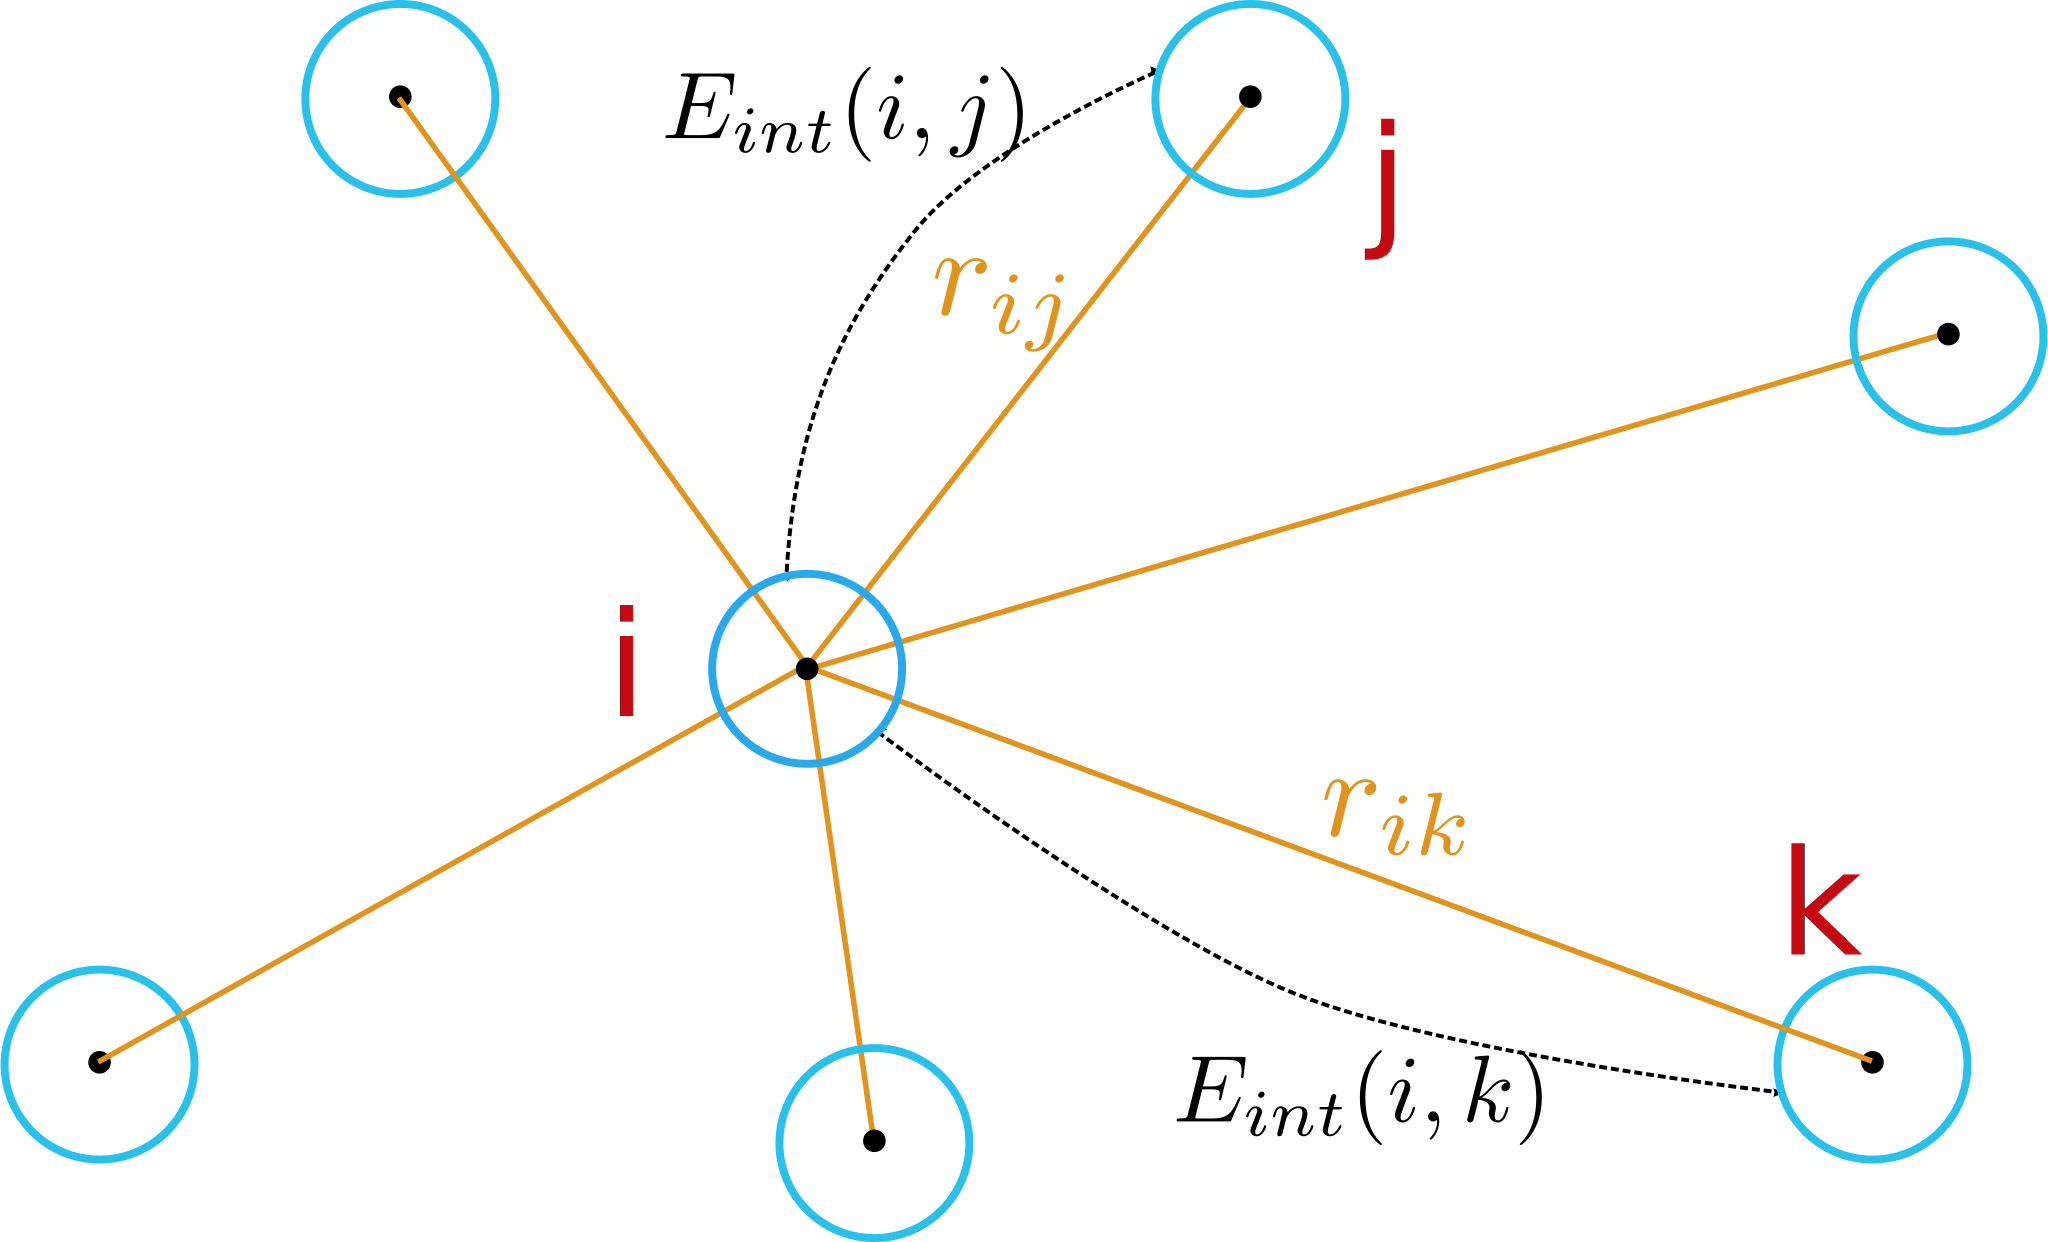
\includegraphics[width=0.6\linewidth]{figures/low_l/Natomes}
\caption[Ensemble de $N$ atomes de Rydberg en interaction Van der Waals]
{Ensemble de $N$ atomes de Rydberg en interaction Van der Waals.
L'énergie d'interaction de chaque atome est la somme de ses énergies d'interaction de paire avec tous les autres.
}
\label{fig:VdW_sum_N}
\end{figure}

	\subsection{Mouvement des atomes au sein d'un gaz dense de Rydberg}
	\noindent Le premier effet des interactions dipolaires au sein d'un nuage d'atomes de Rydberg est un effet mécanique.
Comme nous l'avons vu en \ref{sec:interacting_rydbergs}, l'interaction est répulsive entre atomes de Rydberg dans le même niveau $\ket{\mathrm{nS}}$.
Ainsi, deux atomes de Rydberg en interaction dipolaire subiront chacun une force répulsive, directement dérivée de leur énergie d'interaction,
\begin{equation}
\label{eq:repuls_2atoms}
F = - \frac{d E_{int}}{dr}  = + \frac{6hC_6}{r^7}.
\end{equation}
Cela équivaut à un traitement classique de l'effet mécanique de l'interaction dipolaire, bien que le calcul de cette même interaction ne le soit pas.
Cela nous est permis par la forme simple de l'interaction dipolaire entre deux atomes dans le même état de Rydberg, donnée par l'équation \eqref{eq:Vdd_aa}, qui consiste en un simple déplacement d'énergie du niveau de paire $\ket{aa}$.

Prenons l'exemple de deux atomes dans le niveau $\mathrm{60S}$, séparés d'une distance de $\SI{5}{\um}$ : leur énergie d'interaction vaut $hC_6/r^6 = h\cdot {\SI{137.6}{\GHz\raiseto{6}\um}}/(\SI{5}{\um})^6 = \SI{8.8}{\MHz}$.
Ils se repoussent donc avec une force valant %$6hC_6/r^7 = 6h\cdot \SI{137.6}{\GHz\raiseto{6}\um}/(\SI{5}{\um})^7 = \SI{6.97e-27}{\mega\newton} = \SI{6.97e-21}{\newton}$.
$6hC_6/r^7 =\SI{6.97e-21}{\newton}$.
Étant donnée la masse du rubidium, cette force répulsive correspond à une accélération valant $F/m_{Rb87} = \SI{4.83e4}{\m\per\s\squared}$, soit $\num{5000}$ fois plus que l'accélération de la gravité.
Une intégration numérique grossière permet d'extraire un ordre de grandeur du déplacement des atomes : en $\SI{20}{\us}$, ils auront presque atteint leur vitesse relative maximale de $\SI{0.284}{\m\per\s}$ et en $\SI{10}{\us}$ seulement la distance qui les sépare aura augmenté de $\SI{1.75}{\um}$.
Leur énergie d'interaction aura par là chuté d'un facteur $\SI{5.77}{}$, ce qui constitue une modification considérable du système.

La généralisation à $N$ atomes se fait en additionnant vectoriellement les forces répulsives dues à chaque interaction de paire :
\begin{equation}
\label{eq:repuls_Natomes}
\vec{F}(i) =  \sum_{j\neq i} -\vec{\nabla}E_{int}(i,j)
= \sum_{j\neq i} \frac{6hC_6}{r_{ij}^7} \cdot \frac{-\vec{r}_{ij}}{r_{ij}}
= - 6hC_6 \cdot \sum_{j\neq i} \frac{\vec{r}_{ij}}{r_{ij}^8}.
\end{equation}
%
Cette force répulsive décroît très vite avec la distance.
On s'attend ainsi à ce que deux atomes de Rydberg en interaction s'accélère mutuellement pendant un temps court, se propageant ensuite balistiquement dans des directions opposées.
C'est ce que confirme l'exemple de la paire $\ket{\mathrm{60S,60S}}$ précédemment cité.
Il est intéressant de noter qu'au sein d'un nuage d'atomes de Rydberg, les atomes du c\oe ur  sont repoussés par les interactions dipolaires de tous les côtés.
Les atomes du bord du nuage seront alors expulsés en premier, puis petit à petit les atomes plus au centre pourront commencer à se déplacer.
Le nuage subit ainsi une expansion hydrodynamique non triviale, que nous mesurerons expérimentalement et simulerons numériquement.

	\subsection{Deux régimes d'excitation en interaction dipolaire forte}\label{subsec:excitation_bloc_facil}
	%Le blocage dipolaire et la facilitation}

\noindent Les interactions dipolaires ont également une influence importante sur l'excitation d'un ensemble dense d'atomes de Rydberg.	
En effet, la présence d'un atome de Rydberg conditionne l'excitation ultérieure d'autres atomes de Rydberg dans son voisinage.
Lorsque l'excitation est faite à résonance, cet effet est connu sous le nom de \og blocage dipolaire \fg{}.

	\subsubsection*{Blocage dipolaire et super-atomes}
\noindent Le mécanisme du blocage dipolaire est illustré en figure (\ref{fig:dip_block} a)).
Considérons deux atomes dans l'état fondamental $\ket{g}$, séparés d'une distance $r$.
L'état de la paire est alors $\ket{g,g}$.
Un laser est accordé à résonance pour exciter l'un quelconque de ces deux atomes vers le niveau de Rydberg $\ket{ry}$.
L'état de la paire devient ainsi $\ket{g,ry}$.% ou $\ket{ry,g}$.
Si l'on souhaite exciter le second atome vers le niveau $\ket{ry}$, alors il faut considérer l'énergie nécessaire à la transition $\ket{g,ry} \rightarrow \ket{ry,ry}$.
Or ce dernier état de paire subit un déplacement d'énergie dû à l'interaction de Van der Waals
%
\begin{equation}
\label{eq:DeltaE_block}
\Delta E_{\ket{ry,ry}}(r) = E_{\ket{ry,ry}}(r)-E_{\ket{ry,ry}}(\infty)
= E_{int}(r).
\end{equation}
%
Le laser, qui était à résonance avec la transition $\ket{g,g}\rightarrow\ket{g,ry}$, n'est ainsi plus à résonance avec la transition $\ket{g,ry}\rightarrow\ket{ry,ry}$.
L'excitation du second atome vers un niveau de Rydberg s'en trouve bloquée.

\begin{figure}[!h]
\centering
\includegraphics[height=.3\textheight]{figures/low_l/dip_block}
\caption[Mécanisme du blocage dipolaire]{
Illustration du mécanisme de blocage dipolaire.
\textbf{a)} Diagramme d'énergie des niveaux de paire à zéro, un ou deux atomes excités, en fonction de la distance interatomique $r$.
$\ket{g}$ est le niveau fondamental et $\ket{ry}$ le niveau de Rydberg considéré.
Aux courtes distances, l'interaction dipolaire déplace l'excitation du deuxième atome vers le niveau de Rydberg hors de résonance avec le laser ayant excité le premier atome.
$\gamma$ représente la largeur spectrale de la raie d'excitation à un atome, $E_{int}$ l'énergie d'interaction entre deux atomes de Rydberg et $r_b$ le \og rayon de blocage \fg{}.
\textbf{b)} Généralisation à un ensemble d'atomes. Les points bleus sont des atomes dans l'état fondamental et les points rouges sont des atomes de Rydberg.
Le mécanisme de blocage empêche l'excitation de deux atomes de Rydberg dans un même sphère de rayon $r_b$, représentée par les disques rouges.
}
\label{fig:dip_block}
\end{figure}

Le laser d'excitation n'est pas infiniment fin spectralement et l'effet de blocage dipolaire sera limité par sa largeur spectrale.
On peut en effet considérer que le laser est résonant avec la transition dès lors que le désaccord entre eux est inférieur à la demi-largeur spectrale $\gamma/2$ de la raie d'excitation.
Nous définirons ainsi le \og rayon de blocage \fg{} $r_b$ comme étant la distance en-deçà de laquelle le désaccord est supérieur à la demi-largeur spectrale :
\begin{equation}
\label{eq:def_rayon_bloc}
\Delta E_{int}(r_b) = \gamma /2 
\end{equation}
%
Dans le cas qui nous intéresse, l'interaction dipolaire a une forme de Van der Waals en $1/^6$, permettant de réécrire l'équation \eqref{eq:def_rayon_bloc} sous la forme
\begin{equation}
\label{eq:def_rayon_bloc}
\frac{C_6}{r^6} = \gamma /2 \text{ , soit } r_b = \sqrt[6]{\frac{C_6}{\gamma /2}}
\end{equation}
%
Le mécanisme de blocage est donc effectif à l'intérieur d'un \og volume de blocage\fg{} autour de chaque atome de Rydberg déjà excité.
Ce volume de blocage est une sphère de rayon $r_b$, représentée en figure (\ref{fig:dip_block} b)).

Revenons au cas de deux atomes :
il existe deux états de paire à une excitation, qui sont $\ket{g,ry}$ et $\ket{ry,g}$.
Ces deux états sont dégénérés et le laser couple le niveau fondamental $\ket{g,g}$ indifféremment à $\ket{g,ry}$ et à $\ket{ry,g}$, avec même une fréquence de Rabi $\Omega$.
La combinaison symétrique $\ket{D} = \left( \ket{g,ry} + \ket{ry,g} \right) / \sqrt{2}$, appelée état collectif de Dicke des deux atomes, est alors couplée à l'état fondamental avec une fréquence de Rabi augmentée $\Omega\sqrt{2}$.
Ce facteur d'accroissement a été mis en évidence expérimentalement par le groupe de A. Browaeys et P. Grangier \cite{MX_BROWAEYS_COLLECRABIBLOCK}, en observant deux atomes piégés dans des pinces optiques.

L'idée se généralise au cas à $N$ atomes en utilisant encore une fois le modèle de Dicke.
Dans un rayon de blocage contenant $N_b$ atomes, l'état du système oscille entre l'état fondamental et l'état de Dicke à une excitation, toute excitation supplémentaire étant interdite par blocage dipolaire.
Cette oscillation se fait cette fois avec une fréquence de Rabi $\Omega\sqrt{N_b}$.
Un modèle simple de ce phénomène consiste à voir l'ensemble de ces $N_b$ atomes comme un unique \og super-atome \fg{} ayant un moment de transition dipolaire $\sqrt{N_b}$ plus grand  que celui d'un atome isolé.
Ce modèle de super-atome a été exploité avec succès pour expliquer des observations expérimentales par les groupes d'I. Bloch \cite{MX_BLOCH_SUPERATOM} et de H. Ott \cite{MX_OTT_SUPERATOM}.


	\subsubsection*{Excitation facilitée et agrégats de Rydberg}
	
\begin{figure}[!h]
\centering
\includegraphics[height=.3\textheight]{figures/low_l/dip_facil}
\caption[Mécanisme de facilitation]{
Mécanisme de facilitation
}
\end{figure}

		\noindent les deux régimes d'excitation déterminée par les interactions :\\
		explication du blocage dipolaire, et des effets qui le limitent (ailes de la gaussienne du nuage) \\
		pourquoi c'est difficile dans un BEC : mention du Pfau shift \\
		mention de la négligeabilité des excitations de paires ?

\section{Spectroscopie optique du nuage}
	\subsection{Description de la manip}
		\noindent spectres à différents temps d'interaction\\
		ou $N_rydberg$ en fonction du temps d'interaction pour différents detunings
		
	\subsection{Données : élargissement de la raie laser par interactions}
		\noindent conséquence de la facilitation
		
\section{Modèle de la dynamique d'excitation}
	\subsection{Simulations}
		\noindent modèle d'équation de taux\\
		\noindent résultats de simulations comparés aux manips\\
	\subsection{Les limites du modèle}
		%\noindent question du chauffage
		\noindent photons thermiques et apparition de niveaux $p$ \\
		LIRE T. PORTO
		
\section{Spectroscopie microonde du nuage : voir le mouvement}
	\subsection{Description de la manip}
		\noindent spectroscopie 60s-57s et son spectre d'excitation : comment cela nous donne accès au spectre des énergies d'interaction\\
		sonder le nuage à différents moments de son explosion
	\subsection{Données et accord avec les simulations}
		\noindent présenter les courbes de Raul.IV.3.2
		

\section*{Conclusion}
		\noindent il faut prendre en compte le mouvement, mais aussi les transferts thermiques vers les niveaux $p$
		
%\section{Spectroscopie microonde du nuage}
%	\subsection*{Spectre des énergies d'interaction du nuage}
%		\noindent détails sur la spectro 60s-57s, dont la quasi absence de terme d'échange dans l'interaction
%	\subsection*{Mouvement du nuage de Rydbergs}
%		\noindent Le gaz gelé ne marche pas !

%\chapter{Les atomes de Rydberg circulaires en interaction : vers un simulateur quantique}
%\label{chapter:circsim}
\chapter{Les atomes de Rydberg circulaires en interaction : vers un simulateur quantique}
\label{chapter:circsim}

Intro : pourquoi envisager les Rydberg circulaires comme plateforme de simulation ?

\section{Les interactions dipôle-dipôle entre atomes de Rydberg circulaires}

\section{Le hamiltonien $XXZ$ simulé}
	\subsection{Mise sous forme XXZ}
	\subsection{"Tunabilité" des interactions}
		Comment justifier le domaine de champs électrique et magnétique statiques dans lequel on se place, avant d'avoir parlé du problème de la durée de vie ??
	\subsection{Quelle physique ? Diagramme de phase}

\section{Principes techniques du simulateur}
	\subsection{Piégeage laser des Rydberg circulaires}
	\subsection{Préservation des états de Rydberg}
		\subsubsection*{Temps de vie dans l'espace libre}
		\subsubsection*{Inhibition de l'émission spontanée}
		\subsubsection*{Problème du mixing et solution}
	\subsection{Préparation déterministe d'une chaîne}

\newpage
Reprendre le PRX

%\chapter{Excitation d'atomes de Rydberg circulaires et piégeage laser}
%\label{chapter:50c}
\chapter{Des atomes de Rydberg circulaires sur puce}
\label{chapter:50c}
%Excitation d'atomes de Rydberg circulaires et piégeage laser

\section{Comment exciter des atomes de Rydberg circulaires}
	\subsection*{Les niveaux atomiques du fondamental au Rydberg circulaire}
		\noindent schéma de niveaux et Stark maps
	\subsection*{Spectroscopie 5s-50d}
		\noindent en champ nul et en champ non-nul -> choix de $m_j$
	\subsection*{Spectroscopie 50d-50f}
		\noindent en champ nul et en champ non-nul -> choix de $m_l$ et problème d'élargissement
	\subsection*{Le passage adiabatique}
		\noindent et le dispositif radio-fréquence

\section{Comment caractériser les atomes de Rydberg circulaires}
	\subsection*{Spectroscopie microonde}
		\noindent 50c-51c et optimisation de la RF\\
		\noindent 50c-49c ?
	\subsection*{Temps de vie}
		\noindent temps de vie théorique, temps de vie mesuré, température effective
	\subsection*{Temps de cohérence}
		\noindent franges de Ramsey
	

%\section{Théorie de la force pondéro-motrice appliquée aux 50C} -> goes to chapter:circsim
%	\noindent et description du laser de piégeage

\section{Éjectable : Première évidence du piégeage des atomes circulaires}
	\noindent chute par gravité et/ou expansion du nuage compensée par un tube de lumière


\chapter*{Conclusion}\label{chapter:concl}
\addcontentsline{toc}{chapter}{Conclusion}
\markboth{Conclusion}{Conclusion}
\include{}%0_intro}

%\phantomsection
%\titleformat{\part}[block]
%{\bfseries\fontsize{26}{28}\selectfont}
%{}
%{10pt}
%{
%	\begin{tikzpicture}[remember picture, overlay]
%	\node[anchor=south west, inner sep =0pt, outer sep =25pt](partnum) at (0,3){\partnumfont\itshape };
%	\end{tikzpicture}\parbox[c]{.95\textwidth}%\justify
%}
\part*{Annexes}
\appendix
\renewcommand{\chaptermark}[1]{\markboth{\appendixname\ \thechapter: #1}{}}

\renewcommand{\bibname}{References}
\printbibliography

\include{}%6_appendix}
\backmatter
\include{}%0_intro_fr}
\end{document}